\chapter{Solución}

Una vez nos hemos situado en el contexto en el que se ubica este proyecto, y hemos expuesto los requisitos a cumplir y las herramientas necesarias para llegar a las metas planteadas, nos adentramos a explicar en este capitulo las soluciones utilizadas para llegar a buen puerto.\\

\section{Estructura general}

Como primer problema se presentó decidir cuál de los dos ordenadores que necesitamos para la conexión WebRTC seria el que realizaría la llamada y en que momento del flujo. Este no es un problema trivial, ya que la selección de uno u otro haría que el desarrollo de la aplicación fuese completamente distinto.\\

Se optó por que el par que llevase la batuta de la conexión fuese el ordenador local, ya que este a su vez también es el encargado de  establecer la conexión con el drone. De esta manera tenemos un par que es el que actuará de maestro, estableciendo ambas conexiones en los momentos oportunos.\\

Como ya se comento en la sección \ref{sec:senalizacion} el momento en el que se envía y se recibe cada paquete de información es critico en este sistema de señalización de oferta/respuesta, por lo que el flujo de la comunicación se diseñó y se ha desarrollado como se muestra en la figura \ref{fig:flujodellamada}.\\


\begin{figure}[htb]
\centering
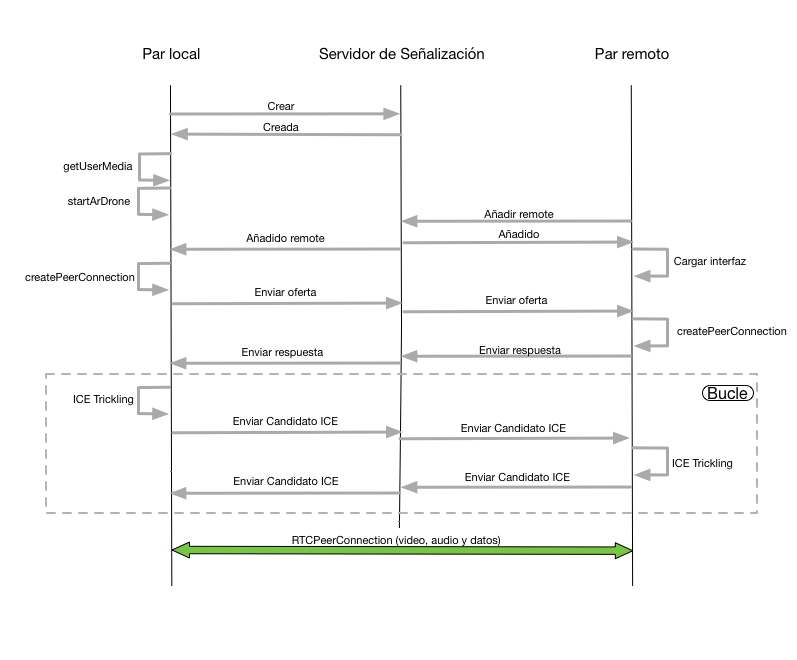
\includegraphics[width=1.1\textwidth]{diagrama_general}
\caption{Flujo de llamada del proyecto}
\label{fig:flujodellamada}
\end{figure}

Como se puede observar el par local es el que lleva la batuta de la conexión. En primer término inicia la comunicación con el servidor de señalización. Una vez que este le contesta afirmativamente a su mensaje de creación de la comunicación inicia un proceso en el que se conecta al cuadricóptero y accede a la cámara. Una vez realizados estos dos procesos espera a que un par remoto quiera unirse a la conexión.\\

Cuando el par remoto accede a servidor de señalización, este le envia un mensaje al par local indicando que un par remoto se ha conectado. En este momento el par local inicia la creación de la conexión \emph{RTCPeerConection} de WebRTC. Primero se produce el intercambio de paquetes SDP a través del servidor de señalización, y posteriormente el de ICE. Una vez finalizados ambos ya tenemos establecida la conexión WebRTC entre ambos pares.\\

\section{Conexión con la API del drone}

Esta primera parte la hemos solucionado dividiendo el problema en dos subproblemas. Por un lado la conexión con el servidor encargado de conectarse al cuadricóptero, \emph{ardone\_server}, y por otro obtener un flujo de vídeo para poder visualizarlo en la parte remota. Este problema lo hemos solucionado incorporando una cámara a bordo del drone que ira conectada al par local y a la cual accederemos desde el navegador con la API getUserMedia que nos brinda WebRTC.\\

Se explica a continuación la conexión con el servidor y posteriormente el acceso a la cámara con getUserMedia.\\


\subsection{ArDrone\_server, ICE y WebSockets}

Para establecer la conexión con el drone se ha utilizado el componente \texttt{ardrone\_server} de JdeRobot. Este componente tiene dos versiones, la componente simulada que es la que hemos instalado en forma de plugin en el simulador Gazebo y la componente real, que se conecta al drone real. Ambas componentes nos ofrecen las mismas interfaces de conexión, por lo que una única configuración de nuestra aplicación bastará para poder trabajar con la versión simulada y la real.\\

En este punto podemos dividir el proyecto en dos partes. Servidor y Cliente. La parte de servidor trataremos básicamente la configuración, y la parte del cliente será la que se desarrolla desde cero.\\

\subsubsection{Servidor}

Los componentes JdeRobot utilizan, como ya hemos visto, interfaces ICE para el intercambio de información del que se ocupan. Los navegadores no tienen capacidad de usar el \emph{middlewre} ICE directamente. Para poder conectarnos con estas interfaces ICE hemos tenido que instalar el plugin ICE for JavaScript, o ICE\-JS. Este plugin nos habilita la opción de conectarnos a estas interfaces directamente desde el navegador usando \emph{websockets}.\\

Aunque estaba disponible la versión 3.6 de ICE\footnote{https://doc.zeroc.com/display/Ice36/Home} la cuál trae en la suite instalado de serie ICE\_JS, hemos usado la versión 3.5, ya que es la versión compatible con la versión más actual de JdeRobot\footnote{http://jderobot.org/Manual-5}. En esta versión ICE\_JS es un plugin a parte el cuál hay que instalarlo descargando el código fuente desde la página de Zeroc\footnote{https://zeroc.com} y compilarlo.\\

Una vez instalado hay que activar este plugin en el servidor. Para ello hay que añadir la siguiente línea en el archivo de configuración del servidor:\\

\begin{lstlisting}[caption=Activación del plugin ICEJS]
# ICE-JS
Ice.Plugin.IceWS=IceWS:createIceWS
\end{lstlisting}

Posteriormente a esto, en el mismo archivo hay que indicarle las direcciones IP y los puertos de cada interfaz de conexión. Cada conexión se corresponderá con un \emph{WebSocket}, y la nomenclatura es la siguiente:\\

\begin{lstlisting}[caption=Formato \emph{endpoints} de los \emph{WebSocket} de ICEJS]
# ICE-JS
:ws -h ip -p puerto
\end{lstlisting}


El servidor tiene hasta un máximo de seis interfaces diferentes a las que te puedes conectar. Cada uno de estas interfaces nos ofrece un servicio diferente. Para nuestro proyecto hemos usado cuatro de esas interfaces.

\begin{itemize}
\item \textbf{Pose3D:} Con esta interfaz accedemos a los datos \emph{pose} del cuadricóptero (x, y, z, h y \emph{quaternion}).
\item \textbf{Navdata:} Esta interfaz nos proporciona los datos de navegación procedentes de los sensores, como la velocidad de las componentes (x, y, z) del drone, altitud, la velocidad del viento, el nivel de batería, etc.
\item \textbf{CMDVel:} Esta interfaz es la que se encarga de recibir las órdenes de movimiento.
\item \textbf{BaseExtra:} Esta interfaz nos da funcionalidades extra como el aterrizaje o el despegue del cuadricóptero.
\end{itemize}

Así pues, esta es la forma final que tiene nuestro archivo de configuración:\\

\begin{lstlisting}[caption=Archivo de configuración]
# Ice-JS
Ice.Plugin.IceWS=IceWS:createIceWS

# Variables de control para ver traceroutes de las conexiones ICE.
#Ice.Trace.Network = 3
#Ice.Trace.Protocol=1


ArDrone.Pose3D.Endpoints=default -h 0.0.0.0 -p 9998:ws -h 0.0.0.0 -p 19000
ArDrone.Pose3D.Name=ardrone_pose3d

ArDrone.RemoteConfig.Endpoints=default -h 0.0.0.0 -p 9997
ArDrone.RemoteConfig.Name=ardrone_remoteConfig

ArDrone.Navdata.Endpoints=default -h 0.0.0.0 -p 9996:ws -h 0.0.0.0 -p 15000
ArDrone.Navdata.Name=ardrone_navdata

ArDrone.CMDVel.Endpoints=default -h 0.0.0.0 -p 9995:ws -h 0.0.0.0 -p 11000
ArDrone.CMDVel.Name=ardrone_cmdvel

ArDrone.Extra.Endpoints=default -h 0.0.0.0 -p 9994:ws -h 0.0.0.0 -p 17000
ArDrone.Extra.Name=ardrone_extra

ArDrone.NavdataGPS.Endpoints=default -h 0.0.0.0 -p 9993
ArDrone.NavdataGPS.Name=ardrone_navdatagps
\end{lstlisting}

A parte de los \emph{endpoints} es también importante configurar correctamente el nombre de cada uno de las interfaces, ya que será necesario para una correcta conexión desde el navegador. La dirección ip \texttt{0.0.0.0} indica que la dirección de escucha del servidor es la ip local del equipo. \\


\subsubsection{Cliente}

Una vez configurado el servidor hemos creado el método ArDrone.js, el cuál es el encargado de conectarse y manejar la conexión con el servidor \texttt{ardrone\_server}.\\

Para establecer una comunicación ICE lo primero es crear las variables ICE necesarias. Estas las creamos de la siguiente manera:\\

\begin{lstlisting}[caption=Formato \emph{endpoints} de los \emph{WebSocket} de ICEJS]
// Variable ICE para la conexion
var id = new Ice.InitializationData();
id.properties = Ice.createProperties();
id.properties.setProperty("Ice.Trace.Network", "3"); // Propiedad para tracear la conexion
id.properties.setProperty("Ice.Trace.Protocol", "1"); // Propiedad para tracear la conexion
var communicator = Ice.initialize(id);
\end{lstlisting}

Por si fallase la comunicación ICE se le ha añadido a la variable \emph{id} una propiedad con la que podemos seguir la ruta de la comunicación y detectar en que punto se produce el fallo.\\

Posteriormente es necesario crear una variable, que será la que actuará como \emph{proxy}, por cada interfaz a la que necesitemos conectarnos. Esta es la nomenclatura que debe seguir:\\

\begin{lstlisting}[caption=Nomenclatura de variable que actuará como \emph{proxy}]
var proxy = communicator.stringToProxy("nombre_interfaz:ws -h " + ip + " -p " + "puerto");
\end{lstlisting}

Nótese en la nomenclatura donde pone \emph{nombre\_interfaz} se corresponde con el nombre que le hemos asignado al \emph{endpoint} en el archivo de configuración del servidor. Asimismo el puerto también se corresponde con el configurado.\\


La comunicación con las interfaces se realiza mediante el objeto promesa o \emph{promise}. Este objeto se usa para las comunicaciones asíncronas y se caracteriza por tener tres estados: pendiente, cumplida o rechazada. Cuando una promesa ha sido llamada puede presentar el estado cumplida o rechazada, lo que nos permite llamar al argumento correspondiente y poder actuar en consonancia. De esta manera podemos hacer que métodos asíncronos actúen como métodos sincronos.\\

El núcleo de la conexión con el servidor \emph{ardrone\_server} queda como sigue:\\

\begin{lstlisting}[caption=Nucleo ArDrone]
// base extra connection
var baseextra = communicator.stringToProxy("ardrone_extra:ws -h " + ip + " -p " + baseextraPort);
jderobot.ArDroneExtraPrx.checkedCast(baseextra).then(
    function(ar){
        extraProxy = ar;
        console.log("extraProxy connected: " + ar);
    },
    function(ex, ar){
        console.log("extraProxy NOT connected: " + ex);
    }
);               

// NavData
var basenavdata = communicator.stringToProxy("ardrone_navdata:ws -h " + ip + " -p " + navdataProxyPort);
jderobot.NavdataPrx.checkedCast(basenavdata).then(
    function(ar){
        console.log("navdataProxy connected: " + ar);
        navdataProxy = ar;
        navdataProxy.getNavdata().then(
        function(navdata){
            if (navdata.vehicle == ARDRONE_SIMULATED) {
                virtualDrone = true;
                console.log("virtualDrone = true");
            } else {
                virtualDrone = false;
                console.log("virtualDrone = false");
            }
        },
        function (ex, ar){
            console.log("Fail getNavdata() function: " + ex);
        }
        );
    },
    function (ex, ar){
        console.log("navdataProxy NOT connected: " + ex);
    }        
);        

// CMDVelPrx
var basecmdVel = communicator.stringToProxy("ardrone_cmdvel:ws -h " + ip + " -p " + cmdVelProxyPort);
jderobot.CMDVelPrx.checkedCast(basecmdVel).then(
    function(ar){
        console.log("cmdVelProxy connected: " + ar);
        cmdVelProxy = ar;
    },
    function(ex, ar){
        console.log("cmdVelProxy NOT connected: " + ex);
    }
);             

// Pose3D
var basepose3D = communicator.stringToProxy("ardrone_pose3d:ws -h " + ip + " -p " + pose3DProxyPort);
jderobot.Pose3DPrx.checkedCast(basepose3D).then(
   function(ar){
       console.log("pose3DProxy connected: " + ar);
       pose3DProxy = ar;
        window.po = pose3DProxy;
        resolve("Stuff worked!");
       pose3DProxy.getPose3DData().then(
           function (ar){
               console.log("getPoseDData().");
               pose = ar;
           },
           function(ex, ar){
               console.log("Fail call getPoseDData().");
           });
   },
   function(ex, ar){
       console.log("pose3DProxy NOT connected: " + ex)
   }
);
\end{lstlisting}

En este punto ya estamos conectados con las interfaces del servidor, y por consiguiente, con el drone. Para poder teleoperar el drone hay que crear unas funciones que serán los manejadores. Por un lado hemos creado las funciones de aterrizaje y de despegue. Estas funciones utilizan la interfaz \emph{ardrone\_extra}:\\

\begin{lstlisting}[caption=Funciones aterrizaje y despegue.º]
// extraProxy functions  
function takeoff() {
    extraProxy.takeoff().then(
        function(ar){
            console.log("Take Off.");
        },
        function(ex, ar){
            console.log("Take Off failed.")
        }
     );
}
    
function land() {
        extraProxy.land().then(
        function(ar){
            console.log("Landing.");
        },
        function(ex, ar){
            console.log("Landing failed: " + ex)
        }
     );
}
\end{lstlisting}

Las interfaces \emph{Navdata} y \emph{Pose3D} so las encargadas de suministrar todos los datos de navegación de los sensores. Las funciones con las que accedemos a estas interfaces y actualizamos todos estos datos son las siguientes:\\

\begin{lstlisting}[caption=Variables actualización datos de los sensores.]

function updateNavData() {
    navdataProxy.getNavdata().then(
        function(ar){
            navdata = ar;
            //console.log("updateNavData()");
        },
        function (ex, ar){
            console.log("Fail getNavdata() function." + ex)
        }        
    );    
}

function updatePose(){
    pose3DProxy.getPose3DData().then(
            function (ar){
                pose=ar;
                //console.log("getPose3DData. ")
            },
            function(ex, ar){
                console.log("Fail call getPoseDData(): " + ar2);
            });   
}

\end{lstlisting}


Llamando a estas funciones periódicamente tenemos actualizados los datos de navegación procedentes de los sensores: brújula, posición, velocidad, altitud...\\

Para poder teleoperar el drone se ha implementado una función que es la encargada de enviarle las órdenes de movimiento.\\

\begin{lstlisting}[caption=Función manejadora de las órdenes.]

function sendVelocities () {
    cmdVelProxy.setCMDVelData(cmd).then(
        function(ar){
          //console.log("sendVelocities.");
        },
        function(ex, ar){
          console.log("sendVelocities failed.")
        }
    );
}

\end{lstlisting}

Dónde la variable \emph{cmd} contiene los parámetros que necesita el drone para moverse. Esta variable es una variable CMDVel de JdeRobot y tiene esta estructura:\\

\begin{lstlisting}[caption=Variable CMD]

var cmd = new jderobot.CMDVelData; 
cmd.linearX=0.0;
cmd.linearY=0.0;
cmd.linearZ=0.0;
cmd.angularZ=0.0;
cmd.angularX=0.0;
cmd.angularY=0.0;

\end{lstlisting}




\subsection{getUserMedia}

La interfaz que no hemos implementado de las que nos ofrece el servidor \texttt{ardrone\_server} es la interfaz \emph{cameraserver}. Esta interfaz se encarga de recoger las imágenes de la cámara integrada en el drone. Para tener una imagen con mas resolución y que nos permita visualizar con mayor calidad se ha optado por colocar una cámara a bordo y acceder a ella con las herramientas que nos suministra WebRTC.\\

Esta camara se conecta a nuestro ordenador local a través de una conexión USB. Camara y MiniPC vana a bordo del drone. Como WebRTC aún no es una norma, para acceder a la cámara desde cualquier navegador debemos crear una variable que sea compatible con todos los que tengan implementado las APIs de WebRTC. Para ello hay que añadirle los prefijos correspondientes de cada navegador:\\


\begin{lstlisting}[caption=Variable de getUserMedia.]
navigator.getUserMedia = navigator.getUserMedia || navigator.webkitGetUserMedia || navigator.mozGetUserMedia;
\end{lstlisting}


Acceder a la cámara a con \emph{GetUserMedia} se hace a través de una función que admite dos llamadas de vuelta o \emph{callback}. Uno de ellos es el callback de éxito, y el segundo el de error. Según sea de exitosa el acceso a la cámara se llamara a una función u otra. Si nos devuelve éxito se llama a una función con la que guardaremos el streaming y lo visualizaremos en un elemento vídeo de HTML5, si devuelve error mostramos un mensaje del error ocurrido.\\

\begin{lstlisting}[caption=getUserMedia.]

// Manejador de exito
function handleUserMedia(stream){
	localStream = stream;

	if (window.URL){
		localVideo.src = window.URL.createObjectURL(stream);
	} else{
		localVideo.src = stream;
	}
	//console.log('Adding local stream.');
	// Envio un mensaje al servidor como ack de exito al llamar gerUserMedia()	
}

// manejador de error
function handleUserMediaError(error){
	console.log('getUserMedia error: ', error);
}

//Funcion getUserMedia
navigator.getUserMedia(constraints, handleUserMedia, handleUserMediaError); 

\end{lstlisting}

El primer argumento de la función es una variable en la que le indicamos las restricciones que queremos: audio, vídeo, solo uno de ellos, resoluciones... Las restricciones elegidas para nuestro proyecto son las siguientes:\\

\begin{lstlisting}[caption=Restricciones de getUserMedia]

var constraints = {
    audio: false,
    video: {
        width: { ideal: 1280, max: 1920 },
        height: {ideal: 720, max: 1080 },
    }
};

\end{lstlisting}

Sólo accedemos al vídeo de la cámara, ya que el audio no lo necesitamos para el proyecto. Por otro lado indicamos una resolución ideal, de 1280x720 píxeles. Si la cámara que le conectamos al ordenador tiene más capacidad restringimos su resolución a HD (1920x1080 píxeles).\\

El flujo que nos proporciona \emph{getUserMedia} lo utilizaremos con \emph{RTCPeerConnection} en para enviárselo al par remoto.\\

\section{Uso WebRTC para el control del drone}

Interconectar el ordenador remoto al drone a través de otro ordenador es el segundo de los objetivos marcados. Para ello vamos a utilizar WebRTC y por su comunicación entre pares. El primer paso es construir un servidor de señalizacion.\\

\subsection{Señalización}

Las necesidades a cubrir en cuanto al servidor de señalización es que sea capaz de intercambiar los datos de red necesarios (Candidatos ICE) y de paquetes SDP. El intercambio debe hacerse con el protocolo de oferta/respuesta según lo establecido en la arquitectura JSEP explicada con anterioridad.\\

Se ha optado por desarrollar el servidor escrito en el lenguaje de programación \emph{Node.js}\footnote{https://nodejs.org/}. Las razones por las que hemos elegido este servidor es que está escrito en JavaScript, por lo que nos resulta muy útil al utilizarse el mismo lenguaje de programación que vamos a utilizar para el resto del proyecto. Por otro lado es un servidor muy liviano.\\

Para cumplir con la arquitectura JSEP vamos a utilizar la librería \emph{Socket.io}\footnote{http://socket.io}, la cuál nos facilita el desarrollo de aplicaciones con necesidades de conexión entre equipos a través de \emph{Websockets}.\\

Como se puede ver en la figura \ref{fig:flujodellamada}, al servidor se le envían 4 tipos de paquetes. Cuando se conecta el par local, cuando se conecta el par remoto, intercambio de candidatos ICE e intercambio de SDP. Sabiendo que tanto los candidatos ICE como los paquetes SDP son objetos, decidimos crear el servidor aceptando tres diferentes tipos de paquetes: el inicial del par local, el inicial del par remoto, y mensajes genéricos que contendrían los objetos anteriormente mencionados. Así pues, esta es la forma del código que gestiona en el servidor el intercambio de paquetes para la señalización.\\

\begin{lstlisting}[caption=Nucleo servidor de señalización]

io.sockets.on('connection', function (socket){

	// Manejaador de mensajes genericos 'message' (intercambios SDP y Candidatos ICE)
	socket.on('message', function (message) {
		//log('Server --> got message: ', message);
		// Si el que envia es Droner hay que mandarlo al remote
		if (socket.id == dronerID) {
			io.sockets.socket(newPeer).emit('message', message);
		// Si el que envia es remote hay que mandarselo al droner
		} else if (socket.id== newPeer) {
			io.sockets.socket(dronerID).emit('message', message);
		} 
	});

	// manejador de mensjes 'create'  enviados por Droner
	socket.on('create', function () {
		//log('Server --> Droner has sido conectado');
		socket.join();
		dronerID = socket.id;
		socket.emit('created');
	});
	

	// Manejador de mensajes 'join remote ' enviados por remote
	socket.on('join remote', function () {
		//log("Server --> Un 'remote' se ha unido.");
		
		io.sockets.in().emit('join remote');
		socket.join();
		newPeer = socket.id;
		socket.emit('joined');
	});
});
\end{lstlisting}

Una vez tenemos el servidor operativo vamos a explicar como hemos creado la conexión entre pares y como hemos usado esta conexion para transmitir el vídeo de la cámara del drone hasta el par remoto.\\

\subsection{RTCPeerConnection: Transmisión de la cámara a bordo}

La conexión entre pares se crea en el momento en el que el par local recibe del servidor de señalizacion un mensaje indicando que el par remoto se ha conectado y esta preparado para crear la conexión. En ese momento se ejecuta una función que configura los parámetros necesarios y  crea la comunicación.\\

Al igual que getUserMedia debemos configurar las variables necesarias para que sean compatibles con todos los navegadores. Para establecer la conexión necesitamos tres variables distintas:\\


\begin{lstlisting}[caption=Variables WebRTC]

RTCPeerConnection = window.RTCPeerConnection || window.mozRTCPeerConnection || 
                       window.webkitRTCPeerConnection || window.msRTCPeerConnection;
RTCPSessionDescription = window.RTCSessionDescription || window.mozRTCSessionDescription ||
                       window.webkitRTCSessionDescription || window.msRTCSessionDescription;
RTCIceCandidate = window.RTCIceCandidate || window.mozRTCIceCandidate ||
                        window.webkitRTCIceCandidate || window.msRTCIceCandidate;

\end{lstlisting}

\begin{itemize}

\item \emph{RTCPeerConnection}: Esta variable es la encargada de crear y mantener la conexión entre pares. Esta variable neesitará de las otras dos para crear la conexión.
\item \emph{RTCPSessionDescription}: Crea los SDP locales y se encarga de gestionar los SDP recibidos.
\item \emph{RTCIceCandidate}: Encargada de descubrir los Candidatos ICE y de gestionar los recibidos del otro par.

\end{itemize}


También debemos indicarle los servidores STUN y TURN a los que conectarse para averiguar los pares de ip y puerto para los Candidatos ICE:\\

\begin{lstlisting}[caption=Servidores STUN y TURN]

var ICE_config = {
  'iceServers': [
    {
      'urls': 'stun:stun.l.google.com:19302'
    },
    {
      'urls': 'stun:23.21.150.121'
    },
    {
      'urls': 'turn:192.158.29.39:3478?transport=udp',
      'credential': 'JZEOEt2V3Qb0y27GRntt2u2PAYA=',
      'username': '28224511:1379330808'
    },
    {
      'urls': 'turn:192.158.29.39:3478?transport=tcp',
      'credential': 'JZEOEt2V3Qb0y27GRntt2u2PAYA=',
      'username': '28224511:1379330808'
    }
  ]
};

\end{lstlisting}

Una vez tenemos las variables configuradas, la forma en la que creamos la conexión WebRTC es la siguiente:\\

\begin{lstlisting}[caption=RTCPeerConnection.]

var PeerConnection = new RTCPeerConnection(ICE_config, pc_constraints);

\end{lstlisting}

Esta función admite dos argumentos. El primero es la configuración ice que ya hemos visto y el segundo es una variable con las restricciones de todas las funcionalidades y configuraciones que tiene RTCPeerConnection. En nuestro caso esa variable está vacía ya que la configuración por defecto es más que adecuada para nuestros intereses.\\

Para que el intercambio de paquetes en la señalización hay que crear los manejadores que RTCPeerConnection necesita para los SDP y para los Candidatos ICE. El par local tiene sus manejadores ya que es el encargado de llevar la batuta de la conexión, y en el par remoto tienen otros manejadores difentes. \\

Los SDP se manejan en el par local con el método \emph{createOffer} que al ser llamado activa el proceso de crear la oferta SDP. Cada vez que crea uno nuevo salta un evento en la función que se le ha indicado, llamada \emph{gotLocalDescription}. Esta función se encarga de ajustar el SDP local al SDP que se acaba de crear y de mandárselo al otro par a través del servidor de señalización. Si al crear un SDP se produce un error se llama a la función de error, la cual se encargara de notificárnoslo en la consola del navegador.\\


\begin{lstlisting}[caption={Manejandor de los SDP.}, label={lst:manejadorsdp}]

// Funcion de exito
function gotLocalDescription(sessionDescription){
  PeerConnection.setLocalDescription(sessionDescription, successLocalSDP, errorLocalSDP);
  sendMessage(sessionDescription);
}

// Funcion de error
function onSignalingError(error){
  console.log('Fallo al crear el SDP: ' + error);	
}

// Metodo manejador de las SDP
PeerConnection.createOffer(gotLocalDescription, onSignalingError);

\end{lstlisting}

Esta oferta es recibida en el par remoto a través del servidor de señalización y se guarda como la oferta del otro par, ya que la necesitaremos para conocer las características del flujo audiovisual que nos llegará:\\


\begin{lstlisting}[caption={Estableciendo SDP del par remoto.}]
PeerConnection.setRemoteDescription(new RTCPSessionDescription(message));
\end{lstlisting}

Al establecer el SDP remoto ocurre un evento del método \emph{createAnswer} y crea una respuesta a la oferta recibida.\\

\begin{lstlisting}[caption=Manejandor de respuestas SDP]
PeerConnection.createAnswer(gotLocalDescription, onSignalingError);
\end{lstlisting}


Las funciones de éxito y error \emph{gotLocalDescription} y \emph{onSignalingError} son las mismas que en el otro par, hemos mostrado su código en el listing \ref{lst:manejadorsdp}.\\

Para manejar los Candidatos ICE utilizamos un método manejador \emph{onicecandidate}, el cuál llama a la función indicada, \emph{handleIceCandidate()}, en el momento en que se encuentra un Candidato ICE. Esta función se encarga de enviar el candidato a través del servidor de señalización. Ambos pares usan este mismo evento con la misma configuración.\\

\begin{lstlisting}[caption=Manejandor de los Candidatos ICE locales.]

function handleIceCandidate(event){
  //console.log('handleIceCandidate event: ', event);
  if (event.candidate) {
    sendMessage({
    type: 'candidate',
    label: event.candidate.sdpMLineIndex,
    id: event.candidate.sdpMid,
    candidate: event.candidate.candidate});
  } else {
    console.log('End of candidates.');
  }
    // console.log('Local ICE candidate: \n' + event.candidate.candidate);
  
}

// Metodo manejador de candidatos ICE
PeerConnection.onicecandidate = handleIceCandidate; // Manejador ICE local (manda ICE local a remoto)

\end{lstlisting}

Los candidatos son recibidos en los pares a través del servidor de señalización. Se crea el candidato y se le añade como candidato remoto con el método \emph{addIceCandidate}.\\

\begin{lstlisting}[caption=Manejandor de los Candidatos ICE remotos.]
var candidate = new RTCIceCandidate({sdpMLineIndex:message.label,candidate:message.candidate});
PeerConnection.addIceCandidate(candidate);
\end{lstlisting}


Uno de los puntos mas importantes para el proyecto que se tiene que encargar \emph{RTCPeerConnection} es transferir el flujo visual desde el par local al par remoto. WebRTC nos lo permite de una forma muy sencilla. En el par local, con un método al que le añadimos como argumento el flujo que hemos obtenido llamar a la API \emph{getUserMedia}:\\

\begin{lstlisting}[caption=Manejandor del flujo audiovisual en el par local.]
PeerConnection.addStream(localStream); 
\end{lstlisting}

Y en el par remoto con un método manejador llamado \emph{onaddstream}, que en el momento de saltar un evento llama a la función \emph{handleRemoteStreamAdded}, y esta se encarga de configurar el flujo en una etiqueta vídeo de HTML5.\\

\begin{lstlisting}[caption=Manejandor del flujo audiovisual en el par remoto.]

// Funcion manejadora
function handleRemoteStreamAdded(event) {
	window.remoteVideo = remoteVideo; // make avalaible on console for inspection
    var remoteVideo = document.getElementById("droneVideo"); // 

	if (window.URL){
		remoteVideo.src = window.URL.createObjectURL(event.stream);
	} else{
		remoteVideo.src = event.stream;
	}
    //console.log('Remote stream attached!!.');
	remoteStream = event.stream;
}

// Metodo manejador 
PeerConnection.onaddstream = handleRemoteStreamAdded;
\end{lstlisting}

Una vez creada y establecida la conexión \emph{RTCPeerConnection} la usaremos para crear la conexión de datos \emph{RTCDataChannel}, para transportar toda la información necesaria hacia ambos lados.\\


\subsection{RTCDataChannel}
\subsubsection{Sensores de navegación}
\subsubsection{Órdenes}
\subsubsection{Localización espacial del drone}


\section{Interfaz amigable y actual}
\subsection{Visualización de las imágenes}
\subsection{Joysticks}
\subsection{Relojes de navegación}